\section*{Experiments}

\subsection*{Data}
A biological dataset is used to evaluate the proposed methods. The DNA of a cell contains genes that are involved in many of the cell's functions. They are often responsible for the production of a protein. The first step in this process is to copy its information to a Messenger RNA (mRNA) strand. To measure how active a specific gene is, we can measure how much of its mRNA we find in the cell.

Genes interact to fulfill a plethora of cell functions. For example, the expression of one gene might up- or down-regulate the expression of some other gene. This interaction is regulated by some biochemical process. 

For a variety of reasons, it is interesting to know how genes interact precisely, that is: what the regulatory network looks like. By jointly measuring the expression of a large set of mRNA strands we obtain an mRNA profile. Collecting a set of these profiles allows us to model the joint distribution of mRNA expression and the causal relations.

Specifically, we use mRNA profiles from \citeauthor{kemmeren2014large}. They measured a profile of 6.182 genes in cells of the yeast species \textit{Saccharomyces cerevisiae} (baker's yeast). The dataset consists of 262 observational samples obtained from unaltered wild type cells, and 1.484 interventional samples obtained from mutant cells where one gene was deactivated.

Both the observational and interventional profiles are reported relatively to some average wild type profile. \citeauthor{kemmeren2014large} report that the interventional profiles are compared to a set of 428 wild type profiles. \silvan{It is unclear if the observational profiles are compared to the same set.}

There are some details of the experiments that might be of relevance in a discussion of underlying assumptions. First of all, the researchers chose to measure only a subset of about 25\% of all genes. Selection criteria included whether genes were expected to be involved in regulating other genes, and only genes were selected that do not play a vital role in keeping the cell alive (viability).

Furthermore, the profile resulting from an experiment had to pass a quality control before being admitted to the dataset. Failing this test resulted either in repeating the experiment, or excluding the mutant. Although these checks improve the quality of the data by removing some failed experiments, they might also admit some selection bias.

A final factor to consider is that  data from previous work of the same institute is included in the dataset, specifically from \citeauthor{lenstra2011specificity} and \citeauthor{van2010functional}. The authors note that they could not find any significant differences in the data. Nevertheless, this information can be seen as a context variable, and ignoring it can be an explicit modelling assumption.

\subsection*{Ground truth}

% GT figure
\begin{figure}[h]
    \centering
    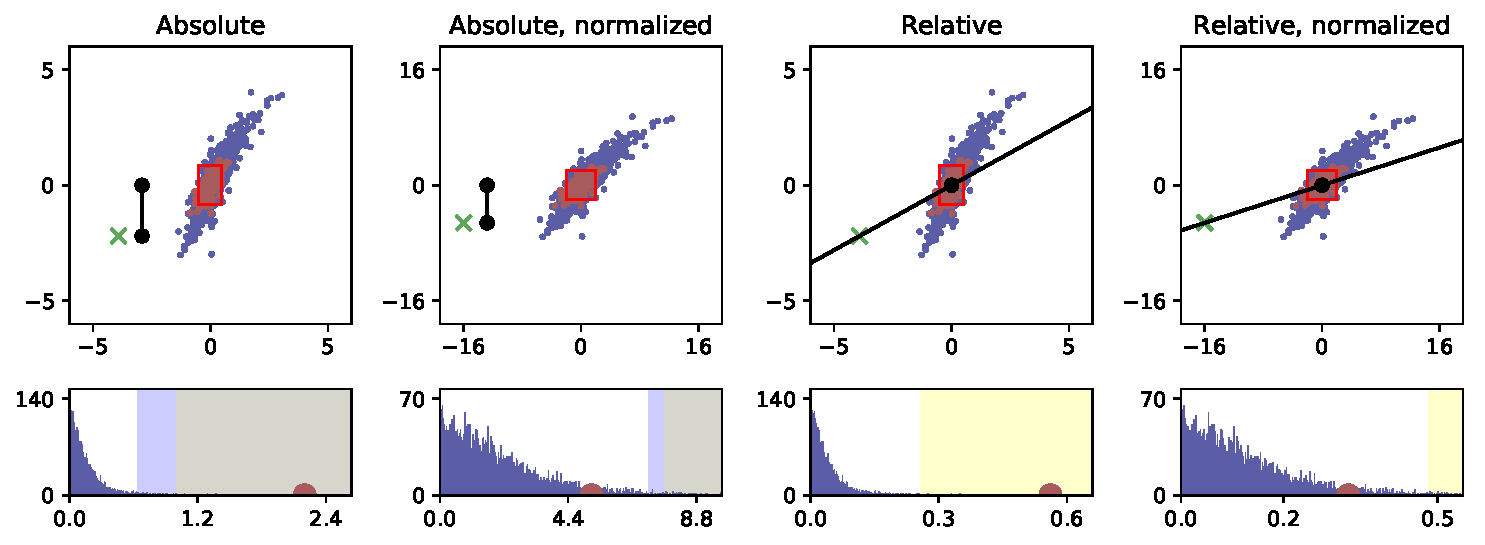
\includegraphics[width=\textwidth]{ground_truth_YHR087W_YDR074W.pdf}
    \caption{
        Different ground-truth definitions illustrated for the knock-out effects of gene YHR087W, particularly on gene YDR074W. TOP: YHR087W on the x-axis and YDR074W on the y-axis for all data points. The green cross indicates the knock-out experiment of YHR087W. The absolute ground-truth is the length of the black line segment, the relative ground-truth is the slope of the black line. The red square indicates a block of 2 standard-deviations in the observed data (red). BOTTOM: distribution of ground-truth scores of all genes in the knock-out experiment of YHR087W. The red half-circle indicates the score of gene YDR074W. The blue plane shows the 99 percentile threshold based on all data, the yellow plane shows it based only on the data from this knock-out experiment. The overlap of both planes is grey.
    }
    \label{fig:ground-truth}
\end{figure}


Value and slope, absolute and 'normalized'

Train-test splits
5-fold cross-validation; separate test set?

\subsection*{Simple analysis}
Visualisation of gene VS gene
Cycles and latent confounders